\newcommand{\wormTagResultsAucTable}{
    \begin{table}[H]
        \centering
        \begin{tabular}{|p{2,8cm}||p{2,8cm} p{2,8cm} p{2,8cm}|}
            \hline
            Worm Tag & ALOHA & Joint Embedding & Proposed Model \\
            \hline
            AUC-ROC & \textBF{0.598$\pm$0.011} & 0.535$\pm$0.017 & 0.534$\pm$0.068 \\
            \hline
        \end{tabular}
        \caption{AUC-ROC (Area Under Curve) of the different models for the \textbf{Worm Tag} prediction task. Results were aggregated over \textBF{3} training runs with different weight initializations and minibatch orderings. Best results are shown in \textbf{bold}.} \label{tab:wormTag_auc}
    \end{table}
}

\newcommand{\wormTagResultsAtFprTable}{
    \begin{center}
        \begin{longtable}[c]{|p{3,2cm}||p{1,8cm} p{1,8cm} p{1,8cm} p{1,8cm} p{1,8cm}|}
            \hline
            Worm Tag & \multicolumn{5}{c|}{{FPR}} \\
            & $10^{-5}$ & $10^{-4}$ & $10^{-3}$ & $10^{-2}$ & $10^{-1}$ \\
            \hline
            \endfirsthead

            \caption*{\raggedright ...continued from previous page} \\
            \hline
            Worm Tag & \multicolumn{5}{c|}{\textbf{FPR}} \\
            & $10^{-5}$ & $10^{-4}$ & $10^{-3}$ & $10^{-2}$ & $10^{-1}$ \\
            \hline
            \endhead

            \caption*{\raggedleft ...continued on next page} \\
            \endfoot

            \caption{Mean and standard deviation results (TPR, Accuracy, Recall, Precision and F1-Score) of the different models for the \textbf{Worm Tag} prediction task at different \textbf{FPR}s (\textit{False Positive Rates}). Results were aggregated over \textBF{3} training runs with different weight initializations and minibatch orderings. Best results are shown in \textbf{bold}. Under \textbf{TPR} results are also presented the percentage reduction in mean detection error and in ROC curve standard deviation introduced by the \textit{Proposed Model} with respect to both \textit{ALOHA} model and \textit{Joint Embedding}.} \label{tab:wormTag_results_at_fpr} \\
            \endlastfoot

            \multicolumn{6}{|c|}{\textbf{TPR}} \\
            \hline
            ALOHA & \textBF{0.001$\pm$0.002} & \textBF{0.001$\pm$0.002} & 0.001$\pm$0.002 & 0.016$\pm$0.003 & 0.145$\pm$0.008 \\
            Joint Embedding & \textBF{0.001$\pm$0.002} & \textBF{0.001$\pm$0.002} & 0.001$\pm$0.002 & \textBF{0.021$\pm$0.010} & \textBF{0.146$\pm$0.029} \\
            Proposed Model & \textBF{0.001$\pm$0.002} & \textBF{0.001$\pm$0.002} & \textBF{0.004$\pm$0.006} & 0.012$\pm$0.008 & 0.132$\pm$0.040 \\
            \hline
            Error Reduction wrt \newline ALOHA & 0.0\% & 0.0\% & 0.3\% & -0.4\% & -1.5\% \\
            Error Reduction wrt \newline Joint Embedding & 0.0\% & 0.0\% & 0.3\% & -0.9\% & -1.6\% \\
            \hline
            Std Reduction wrt \newline ALOHA & 0.0\% & 0.0\% & -200.0\% & -166.7\% & -400.0\% \\
            Std Reduction wrt \newline Joint Embedding & 0.0\% & 0.0\% & -200.0\% & 20.0\% & -37.9\% \\
            \hline
            \multicolumn{6}{|c|}{\textbf{Accuracy}} \\
            \hline
            ALOHA & \textBF{0.896$\pm$0.000} & \textBF{0.896$\pm$0.000} & \textBF{0.895$\pm$0.000} & \textBF{0.889$\pm$0.000} & 0.821$\pm$0.001 \\
            Joint Embedding & \textBF{0.896$\pm$0.000} & \textBF{0.896$\pm$0.000} & 0.895$\pm$0.001 & 0.889$\pm$0.001 & \textBF{0.822$\pm$0.003} \\
            Proposed Model & \textBF{0.896$\pm$0.000} & \textBF{0.896$\pm$0.000} & \textBF{0.895$\pm$0.000} & 0.888$\pm$0.001 & 0.820$\pm$0.004 \\
            \hline
            \multicolumn{6}{|c|}{\textbf{Recall}} \\
            \hline
            ALOHA & \textBF{0.001$\pm$0.002} & \textBF{0.001$\pm$0.002} & 0.001$\pm$0.002 & 0.016$\pm$0.003 & 0.145$\pm$0.008 \\
            Joint Embedding & \textBF{0.001$\pm$0.002} & \textBF{0.001$\pm$0.002} & 0.001$\pm$0.002 & \textBF{0.021$\pm$0.010} & \textBF{0.146$\pm$0.029} \\
            Proposed Model & \textBF{0.001$\pm$0.002} & \textBF{0.001$\pm$0.002} & \textBF{0.004$\pm$0.006} & 0.012$\pm$0.008 & 0.132$\pm$0.040 \\
            \hline
            \multicolumn{6}{|c|}{\textbf{Precision}} \\
            \hline
            ALOHA & \textBF{1.000$\pm$0.000} & \textBF{1.000$\pm$0.000} & \textBF{0.333$\pm$0.471} & 0.163$\pm$0.025 & 0.144$\pm$0.007 \\
            Joint Embedding & \textBF{1.000$\pm$0.000} & \textBF{1.000$\pm$0.000} & \textBF{0.333$\pm$0.471} & \textBF{0.197$\pm$0.085} & \textBF{0.145$\pm$0.025} \\
            Proposed Model & \textBF{1.000$\pm$0.000} & \textBF{1.000$\pm$0.000} & 0.167$\pm$0.236 & 0.116$\pm$0.071 & 0.132$\pm$0.036 \\
            \hline
            \multicolumn{6}{|c|}{\textbf{F1 Score}} \\
            \hline
            ALOHA & \textBF{0.003$\pm$0.004} & \textBF{0.003$\pm$0.004} & 0.003$\pm$0.004 & 0.029$\pm$0.006 & 0.144$\pm$0.008 \\
            Joint Embedding & \textBF{0.003$\pm$0.004} & \textBF{0.003$\pm$0.004} & 0.003$\pm$0.004 & \textBF{0.038$\pm$0.017} & \textBF{0.146$\pm$0.027} \\
            Proposed Model & \textBF{0.003$\pm$0.004} & \textBF{0.003$\pm$0.004} & \textBF{0.008$\pm$0.011} & 0.021$\pm$0.015 & 0.132$\pm$0.038 \\
            \hline
        \end{longtable}
    \end{center}
}

\newcommand{\wormTagResultsSummaryTable}{
    \begin{table}[H]
        \centering
        \begin{tabular}{|p{3,2cm}||p{1,8cm} p{1,8cm} p{1,8cm} p{1,8cm} p{1,8cm}|}
            \hline
            \multicolumn{6}{|c|}{Worm Tag (at FPR $=1\%$)} \\
            \hline
            Model & TPR & Accuracy & Precision & Recall & F1 score \\
            \hline
            ALOHA & 0.016$\pm$0.003 & \textBF{0.889$\pm$0.000} & 0.163$\pm$0.025 & 0.016$\pm$0.003 & 0.029$\pm$0.006 \\
            Joint Embedding & \textBF{0.021$\pm$0.010} & 0.889$\pm$0.001 & \textBF{0.197$\pm$0.085} & \textBF{0.021$\pm$0.010} & \textBF{0.038$\pm$0.017} \\
            Proposed Model & 0.012$\pm$0.008 & 0.888$\pm$0.001 & 0.116$\pm$0.071 & 0.012$\pm$0.008 & 0.021$\pm$0.015 \\
            \hline
        \end{tabular}
        \caption{Summary of the mean and standard deviation results of the different models for the \textbf{Worm Tag} prediction task at \textbf{FPR} $=1\%$. Results were aggregated over \textBF{3} training runs with different weight initializations and minibatch orderings. Best results are shown in \textbf{bold}.} \label{tab:wormTag_result_summary}
    \end{table}
}

\newcommand{\wormTagRocAloha}{
    \begin{figure}[H]
        \vspace*{-0.5cm}
        \centering
        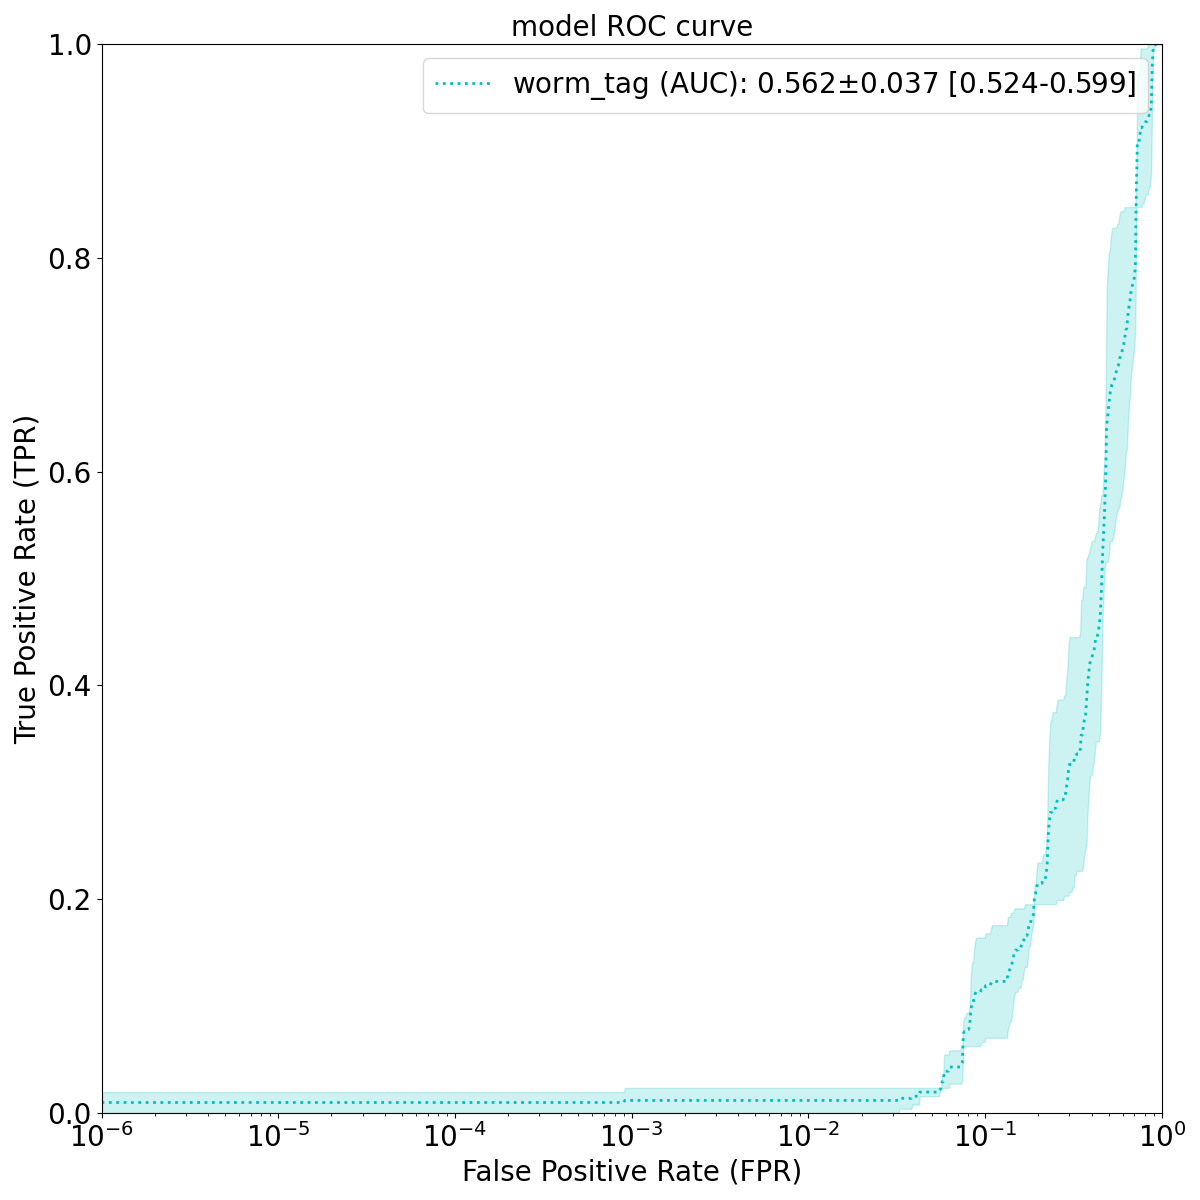
\includegraphics[width=0.6\textwidth]{./results/worm_tag_roc_aloha.png}
        \vspace*{-0.2cm}
        \caption{ROC curve and AUC statistics of \textBF{ALOHA} model for the \textbf{Worm Tag}. The line represents the \textit{mean} TPR at a given FPR, while the shaded region represents the \textit{standard deviation}. Statistics were computed over \textBF{3} training runs, each with random parameter initialization.}
        \label{fig:wormTagRocAloha}
    \end{figure}
}

\newcommand{\wormTagRocJointEmbedding}{
    \begin{figure}[H]
        \vspace*{-0.5cm}
        \centering
        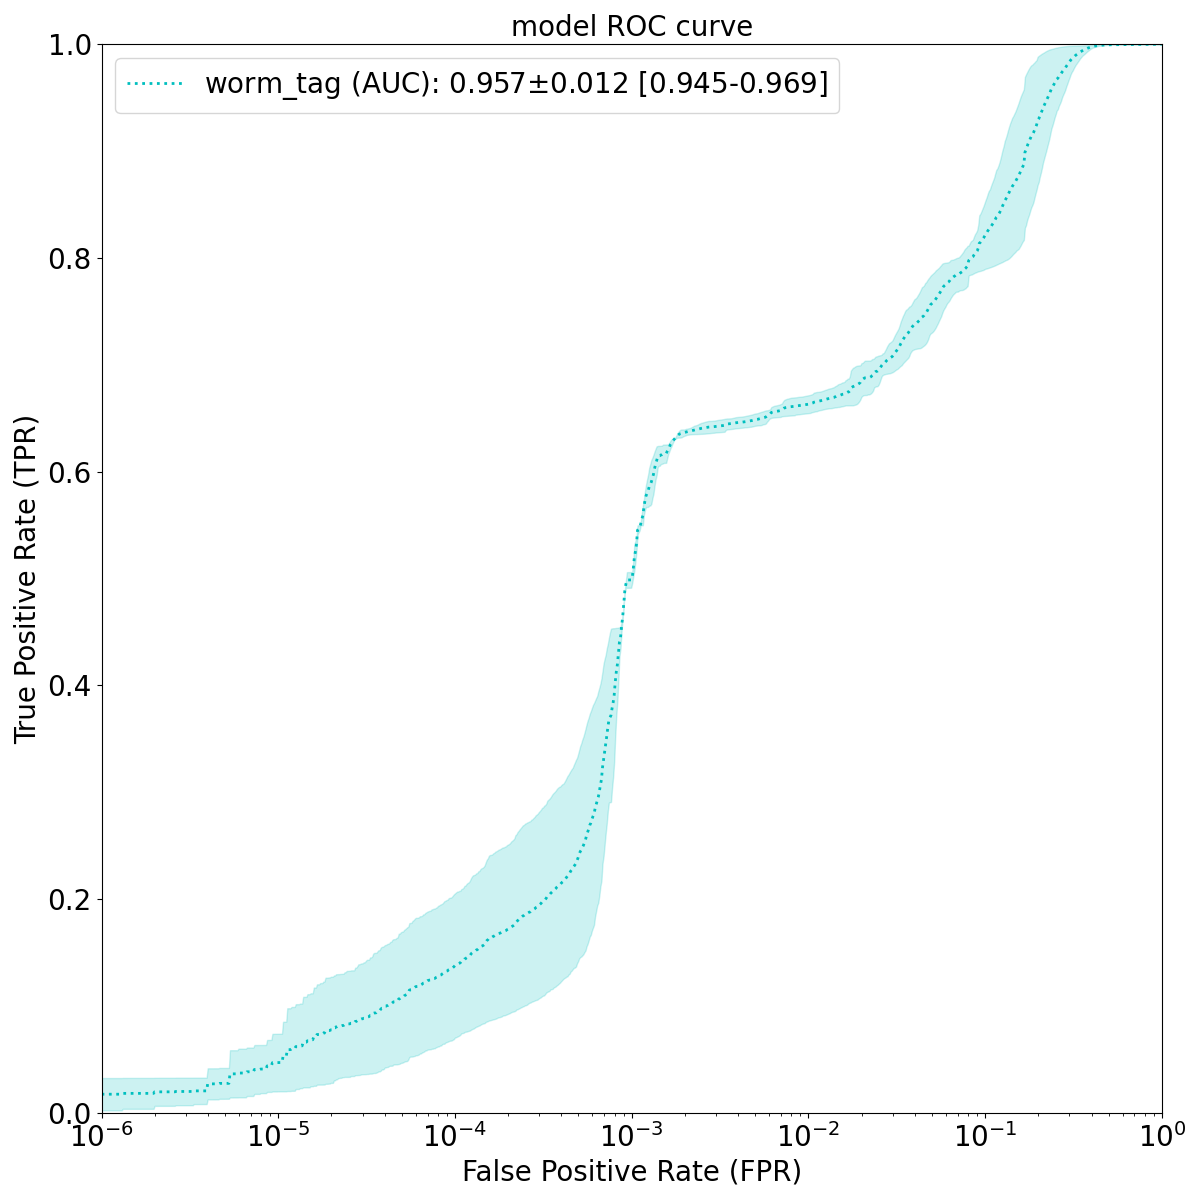
\includegraphics[width=0.6\textwidth]{./results/worm_tag_roc_jointEmbedding.png}
        \vspace*{-0.2cm}
        \caption{ROC curve and AUC statistics of \textBF{Joint Embedding} model for the \textbf{Worm Tag}. The line represents the \textit{mean} TPR at a given FPR, while the shaded region represents the \textit{standard deviation}. Statistics were computed over \textBF{3} training runs, each with random parameter initialization.}
        \label{fig:wormTagRocJointEmbedding}
    \end{figure}
}

\newcommand{\wormTagRocProposedMethod}{
    \begin{figure}[H]
        \vspace*{-0.5cm}
        \centering
        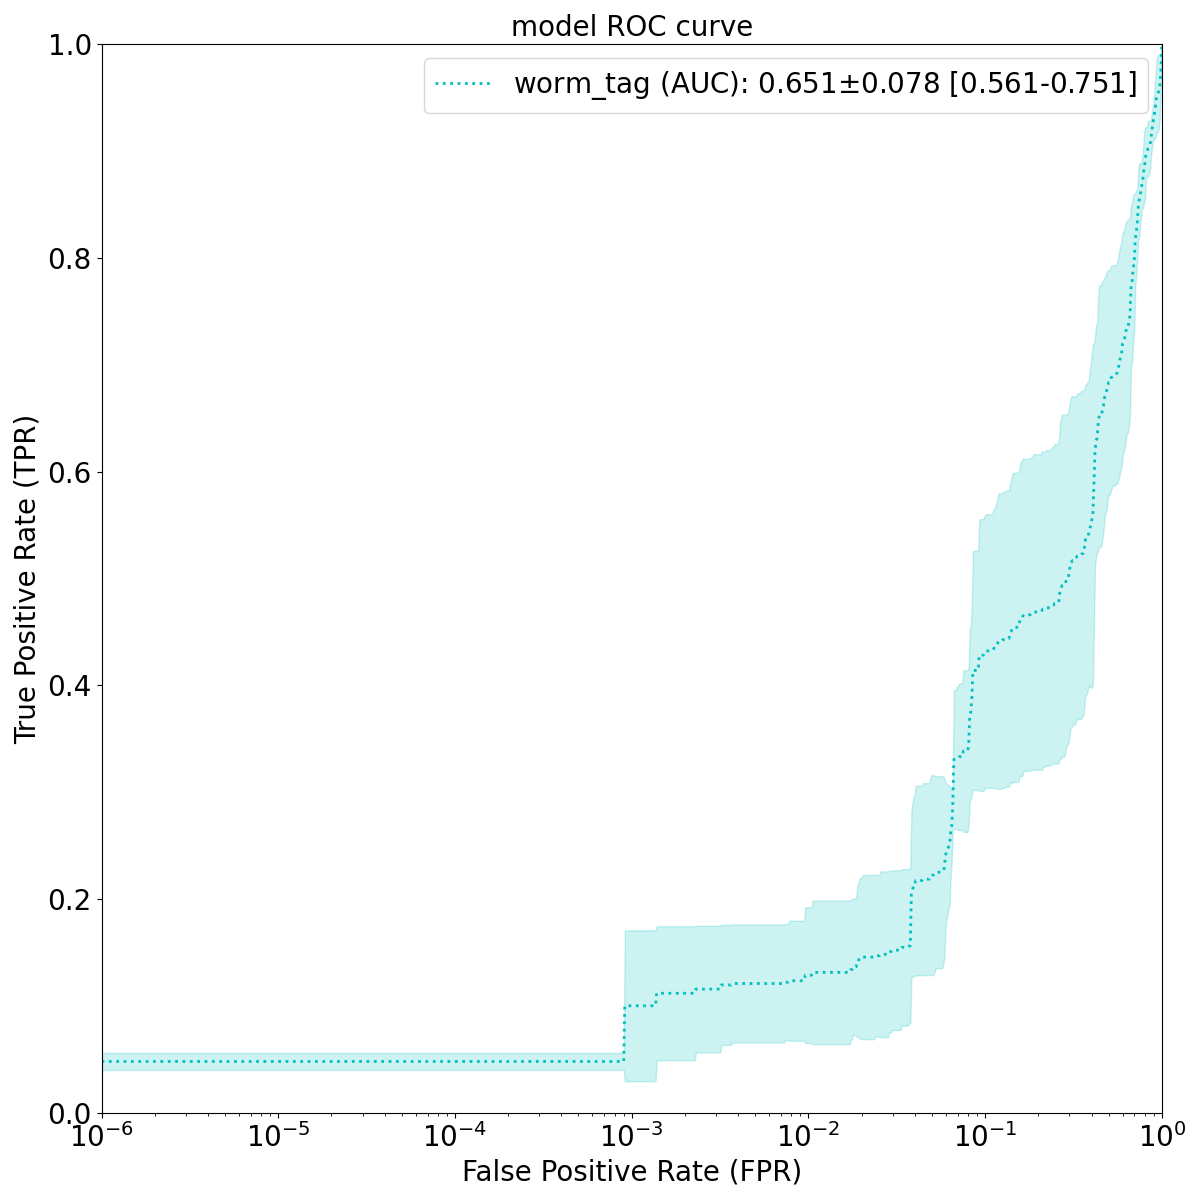
\includegraphics[width=0.6\textwidth]{./results/worm_tag_roc_proposedModel.png}
        \vspace*{-0.2cm}
        \caption{ROC curve and AUC statistics of \textBF{Proposed Model} for the \textbf{Worm Tag}. The line represents the \textit{mean} TPR at a given FPR, while the shaded region represents the \textit{standard deviation}. Statistics were computed over \textBF{3} training runs, each with random parameter initialization.}
        \label{fig:wormTagRocProposedModel}
    \end{figure}
}
